\fancyhf{}
\pagestyle{fancy}
%Encabezado
\lhead[]{\leftmark}
\chead[]{}
\rhead[]{\thepage}
\renewcommand{\headrulewidth}{1pt}

\section{Introducción}

En el capítulo anterior, se explicó la importancia de analizar ids ubicados en los códigos. Los ids ocultan información que es propia del Dominio del Problema (ver capítulo 3). Desafortunadamente, las personas ajenas al código, no comprenden a simple vista la información que los ids poseen e invierten tiempo en entender su presencia en el código. Es por esto, que las herramientas automáticas de análisis de ids son bienvenidas en el ámbito de la Comprensión de Programas (CP). Con estas herramientas se logra achicar los tiempos de comprensión de ids y revelar la información poco visible que estos contienen.

Dada la importancia que tienen las herramientas de análisis de ids, se tomó la iniciativa de desarrollar una llamada Identifier Analyzer (IDA). Esta herramienta le permite al usuario ingresar un archivo JAVA, luego IDA analiza los ids que están en el archivo, y finalmente muestra como resultado una tabla del análisis realizado.
El objetivo de IDA es lograr que el usuario comprenda más rápidamente el propósito de los ids en los archivos JAVA, y de esta manera mejorar la comprensión del código analizado.

%Para que IDA pueda realizar su tarea, contiene implementados 2 algoritmos de división de ids (Greedy y Samurai) y 1 algoritmo de expansión de abreviaturas (Expansión Básica), los mismos fueron explicados en el capítulo precedente. 

El correspondiente capítulo, está destinado a explicar los distintos módulos que IDA posee, y que proceso de ejecución debe realizar el usuario para analizar los ids. Al final de este capítulo, se describen algunos casos de estudio que demuestran la importancia de haber construido IDA. Todas estas explicaciones, están acompañadas con capturas de pantalla y tablas que facilitarán al lector entender el funcionamiento de la herramienta IDA. 
Para comenzar con la descripción de IDA, en la siguiente sección se explica la arquitectura y cuales son sus componentes principales.

%La herramienta IDA le permite al usuario ingresar archivos con código JAVA. Luego la herramienta ejecuta técnicas/algoritmos que analizan los ids situados en el código del archivo.

%La herramienta IDA le permite al usuario revelar la información estática oculta que hay detrás de los ids. Esto se logra mediante la ejecución de técnicas/algoritmos que fueron descriptos en el capítulo anterior.
%
%La iniciativa del desarrollo de la herramienta IDA surgió, porque en la actualidad no existe otra herramienta en el ámbito de la CP con similares características.

%El objetivo de aplicar estas técnicas consiste en convertir los ids que están abreviados a palabras completas más entendibles para el lector ajeno al código.

%Una vez realizada esta conversión, IDA le permite al usuario reemplazar a elección los ids con los nuevos nombres, creando así un nuevo archivo con código más legible y sin alterar la funcionalidad original del código. 

\begin{figure}[t] %[h] para here [b] para bottom [t] para top
\centerline{%queda centrada mejor la imagen
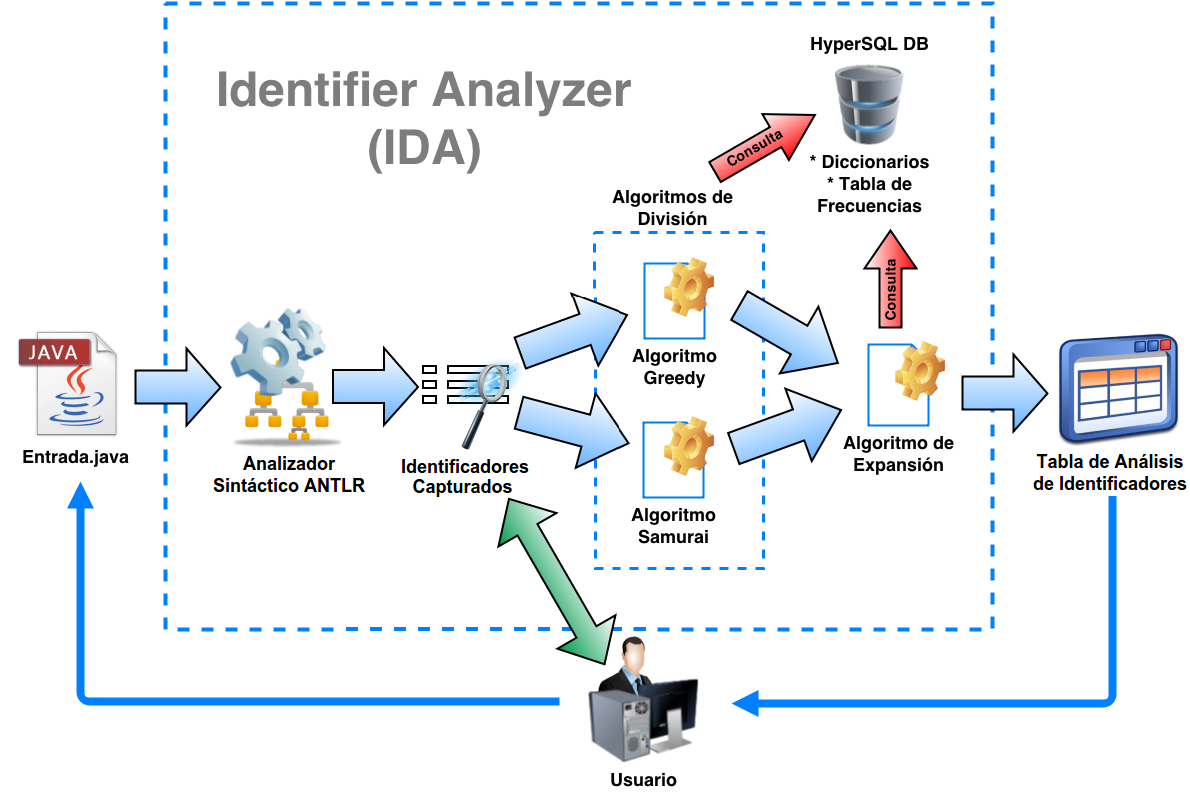
\includegraphics[scale= 0.35]{./cap4/ida_arq.png}
}
\caption{Arquitectura de IDA.}
\label{arq1}
\end{figure}


\section{Arquitectura}

%La herramienta IDA se implementó empleando lenguaje JAVA y se programó usando el entorno de desarrollo NetBeans\footnote[1]{https://www.netbeans.org}. 

En la figura \ref{arq1} se puede apreciar la arquitectura de IDA. Esta arquitectura describe tres partes principales, la primera consiste en la \textit{extracción de datos}, la segunda trata sobre la \textit{división de ids} y la tercera sobre \textit{expansión de ids}. A continuación se detallan cada una de ellas.\\

\textbf{Módulo de Extracción de Datos:} Este módulo recibe como entrada un archivo JAVA que ingresa el usuario (ver Figura \ref{arq1} Entrada.java), luego este archivo se procesa por un Analizador Sintáctico (AS) (\mbox{ver Figura \ref{arq1}} Analizado Sintáctico ANTLR). El AS, extrae y almacena en estructuras internas la información estática perteneciente al código del archivo ingresado. Esta información extraída, está relacionada con ids, literales y comentarios (ver próxima sección para más detalles). El usuario a través de la interfaz de IDA, puede visualizar esta información capturada del código por medio de tablas claramente definidas (ver figura \ref{arq1} - Flecha Verde).

\textbf{Módulo de División de Ids:} Una vez completada la extracción de información, el proceso continua en el módulo de división de ids. Aquí se encuentran implementados 2 algoritmos de división; uno es el Algoritmo Greedy y el otro es el Algoritmo Samurai ambos explicados en el capítulo anterior. Estos algoritmos reciben como entrada la información capturada en el módulo de extracción de datos (ids, comentarios, literales), luego estos algoritmos se encargan de dividir los ids del archivo JAVA (ver figura \ref{arq1} Algoritmos de División). Los resultados de las divisiones se almacenan en estructuras internas que serán utilizadas en próximo módulo. Cabe recordar que estos algoritmos de división necesitan datos externos para funcionar, uno es el diccionario de palabras (en caso de Greedy) y el otro es lista de frecuencias globales de aparición de palabras (en caso de Samurai). Estos datos externos se encuentran almacenados en una base de datos embebida (parte superior de la figura \ref{arq1} - Flechas Rojas).

\textbf{Módulo de Expansión de Ids:} La tercera y última parte, tiene implementado el Algoritmo de Expansión Básico de abreviaturas que fue explicado en el capítulo anterior. Este algoritmo toma como entrada los ids divididos en la etapa anterior, tanto de Greedy como de Samurai. Luego, el Algoritmo de Expansión procede a expandir los ids obtenidos por estos 2 algoritmos, dando como resultado ids expandidos desde Greedy y desde Samurai (ver figura \ref{arq1} Algoritmo de Expansión). 
%En este punto, el usuario podrá elegir que expansión es la más adecuada y reemplazar los ids originales en el archivo de entrada, generando de esta manera un nuevo archivo de salida (ver figura \ref{arq1} Salida.java). 
El \mbox{Algoritmo} de Expansión también necesita de un diccionario de palabras, por eso se realizan consultas a la base de datos embebida (parte superior de la figura \ref{arq1} - Flechas Rojas). Finalmente, los resultados de las divisiones y las expansiones de los ids, son exhibidas en una tabla (ver figura \ref{arq1} Tabla de análisis).

\section{Analizador Sintáctico}

Como se explicó en la sección previa, cuando el usuario ingresa un archivo JAVA, IDA utiliza un Analizador Sintáctico (AS) que examina y extrae información estática presente en el archivo ingresado. Esta información está compuesta por identificadores, comentarios y literales.

La construcción de este AS se llevó a cabo, primero investigando herramientas encargadas de construir AS. Se dio preferencia a aquellas que emplean la teoría asociada a las gramáticas de atributos \cite{AHUL06}. De la investigación previamente descripta, se determinó que la herramienta \textit{ANTLR}\footnote[1]{ANother Tool for Language Recognition. http://www.antlr.org} era la que mejor se ajustaba a las necesidades antes planteadas. 
Esta herramienta permite agregar acciones semánticas (escritas en JAVA) para el calculo de los atributos, en una gramática de lenguaje JAVA\footnote[2]{Especificaciones de la gramática JAVA en http://docs.oracle.com/javase/specs/jls/se7/jls7.pdf}. Estas acciones semánticas deben estar correctamente insertadas en la gramática para, por ejemplo, implementar estructuras de datos y algoritmos que capturan los ids utilizados en un programa \cite{AAJU83}. Una vez insertadas estas acciones, ANTLR se encarga de leer la gramática y generar el AS adicionando acciones que fueron programadas. De esta manera, se obtiene un AS que recolecta ids mientras examina el código. A su vez a estas acciones semanticas, se le agregan otras acciones que extraen comentarios y literales strings. Estos elementos son necesarios ya que sirven para los algoritmos de análisis de ids que serán explicados en próximas secciones.

\section{Base de Datos  Embebida}
\label{sec:bseEmb}

Dado que IDA necesita de diccionarios y listas de palabras para poder llevar a cabo sus tareas, los mismos están almacenadas dentro de IDA en una base de datos embebida. 
Esta base de datos utiliza una tecnología llamada HSQLDB\footnote[3]{Hyper SQL Data Base. http://www.hsqldb.org} y al estar desarrollada en JAVA permite una correcta integración con IDA.
Otra ventaja que tiene esta tecnología es que responde rápidamente las consultas.

A continuación, se describen los diccionarios/listas de palabras que están alojadas en la base de datos explicada en el párrafo anterior. También se nombran los algoritmos implementados en IDA que consultan cada una.

\begin{description}
\itemsep0em%reduce espacio

\item[Diccionario en Inglés (ispell):] Contiene palabras en Inglés que pertenecen a la lista de Palabras de \textit{Ispell}\footnote[1]{Comando de Linux. http://wordlist.aspell.net}. Se utiliza en el Algoritmo de Greedy y en el Algoritmo de Expansión (ver capítulo 3).

\item[Lista de Palabras Excluyentes (stop-list):] Esta compuesta con palabras que son poco importantes o irrelevantes en el análisis de ids. Se utiliza en el Algoritmo de Greedy y en el Algoritmo de Expansión \mbox{(ver capítulo 3)}.

\item[Lista de Abreviaturas y Acrónimos Conocidas:] Contiene abreviaturas comunes del idioma Inglés y Acrónimos conocidos de programación (gif, jpg, txt). Se emplea en el Algoritmo Greedy (ver capítulo 3).

\item[Lista de Prefijos y Sufijos Conocidos:] Posee Sufijos y Prefijos conocidos en Inglés, esta lista fue confeccionada por el autor del Algoritmo Samurai (ver capítulo 3). Se consulta solo en dicho algoritmo.

\item[Frecuencias Globales de Palabras:] Lista de palabras, junto con su frecuencia de aparición. Esta lista fue construida por el autor del Algoritmo Samurai. Se emplea solo en dicho algoritmo, más precisamente en la función de \textit{Scoring} (ver capítulo 3).

\end{description}

Cabe destacar que las listas y diccionarios que fueron descriptos poseen palabras que pertenecen al idioma Inglés, dado que los autores así lo determinaron. Por lo tanto, para que la herramienta IDA analice correctamente los ids, se recomienda ingresar en IDA archivos JAVA con comentarios, literales e ids acordes a la lengua Inglesa. 

Habiendo descripto los principales módulos de la herramienta, en la próxima sección se explicará el proceso que debe seguir el usuario para analizar ids a través de IDA.